\clearpage
\section{Introduction}
\label{sec:Intro}

\subsection{A global picture of the Universe}

\begin{wrapfigure}{l}{0.6\linewidth}
	\centering
	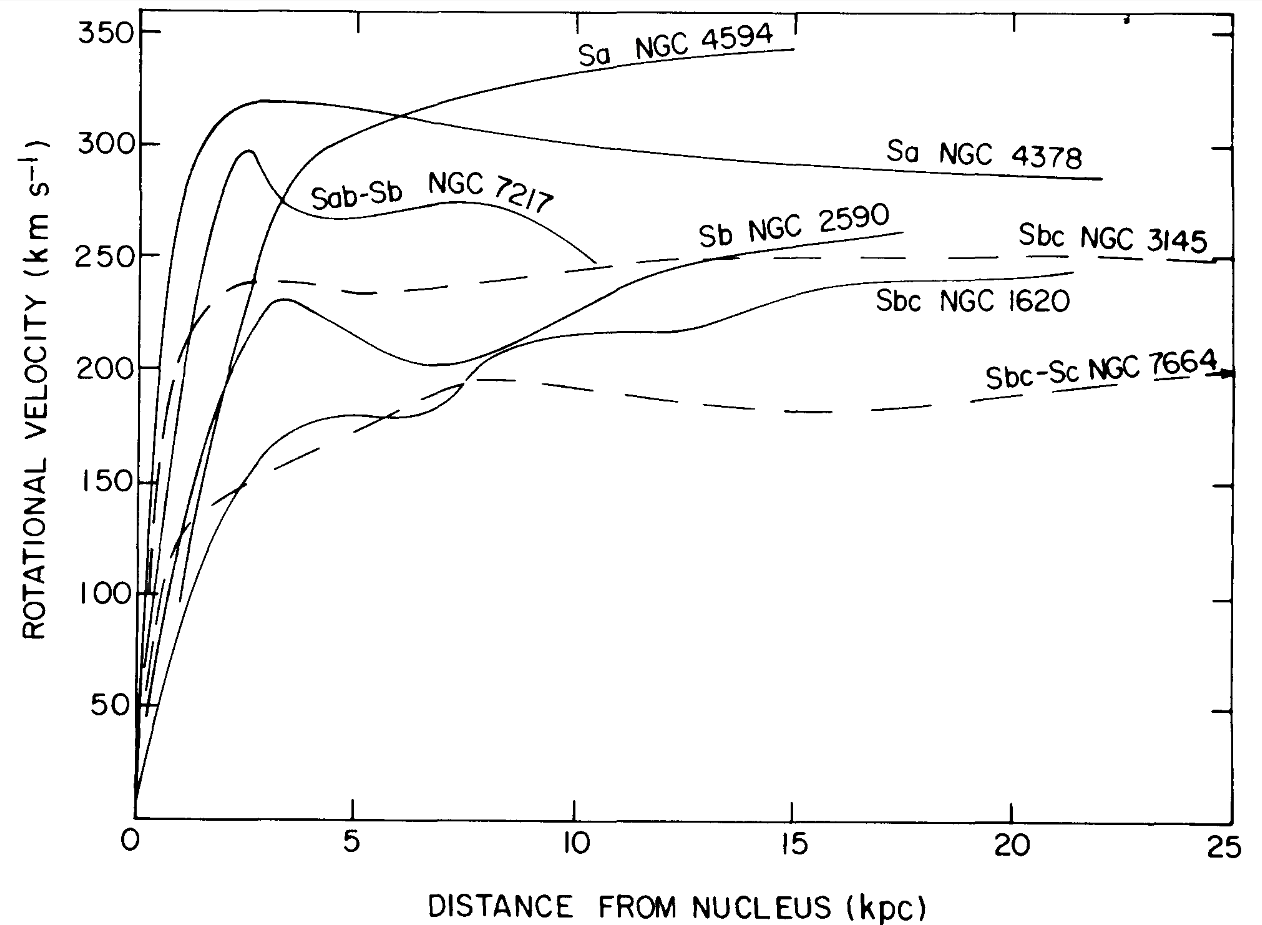
\includegraphics[width=\linewidth]{{Figures/Rubin1978}}
	\caption[Rotation curves from Vera Rubin]{Rotation curves of $7$ spiral galaxies observed by Vera C. Rubin, W. Kent Ford, Jr, and Norbert Thonnard \shortcite{Rubin1978}. These were among the first measurements which unveiled the presence of dark matter around galaxies.}
	\label{fig:RotRubin}
\end{wrapfigure}

Our knowledge of galaxy properties and their evolution through cosmic time has drastically changed from the early 20th century when the Grand Debate \shortcite{GrandDebate} between Harlow Shapley and Heber Curtis on the (extra)galactic origin of the so-called nebulae took place (see \shortciteA{Trimble1995} for an interesting discussion on the subject). Since \shortciteA{Hubble1926}, \shortciteA{Hubble1929} measurements of these nebulae distances to us, we know they actually are galaxies like our own lying at great distances and moving away from us. This global movement was understood in the cosmological framework of an expanding Universe. In a few months of interval, in 1998-1999, two teams measured the redshift and distance of far distant type Ia supernovae, considered as standard candles, and held evidence for an accelerating expansion which revived the need of a cosmological constant in Einstein's field equations \shortcite{Riess1998}, \shortcite{Perlmutter1999}. This additional term has been interpreted as a fluid with negative pressure acting against gravity, and is known as dark energy. Additionally, the first evidence of a dark component in galaxy clusters mass distribution was suggested by Fritz Zwicky \shortcite{Zwicky1933}, \shortcite{Zwicky1937}. By measuring the relative velocity of $7$ galaxies in Coma Berenices, he derived a velocity dispersion $\sigma_{\rm{v}}$ from which he computed with the virial theorem an order of magnitude for the cluster dynamical mass $M_{\rm{d}} \sim (\sigma_{\rm{v}}^2 R ) / G$, with $R$ the cluster characteristic size. The given mass was roughly two orders of magnitude above the expected luminous mass from the luminosity of the galaxies. However, this argument never really convinced the other astronomers at the time. A stronger proof for the existence of a dark component embedded in galaxies came from the study of galaxy rotation curves performed by Vera Rubin in the 1970s \shortcite{Rubin1970}, \shortcite{Rubin1978}. By looking at the outer material of galaxies, she observed flat rotation curves which either indicated a deviation from Newton's law of gravitation or the presence of large amounts of dark matter in surrounding haloes. \\

From this point onward, the need of a unified cosmological model including these new aspects became obvious. Decades of observations, state of the art N-body simulations and measurements of cosmological probes have given the actual $\Lambda \rm{CDM}$ model its renown. In the meantime, as cosmology advanced and the size of the Universe exploded following Hubble 1929 publication, a new branch of astronomy centred on galaxies quickly developed both in terms of observations and of theoretical modelling.


\subsection{What we have learned about galaxies so far}

\subsubsection{Evolving properties with redshift ?}

Nowadays, galaxies are understood as gravitationally bound collections of stars, gas and dust which are supposed to have collapsed from initial clouds embedded in rapidly growing dark mater haloes. Galaxies formation and evolution should therefore follow the growth of the dark matter distribution through space and time, and as such should be tightly correlated to the global properties of our Universe. \\

\begin{wrapfigure}{r}{0.55\linewidth}
	\centering
	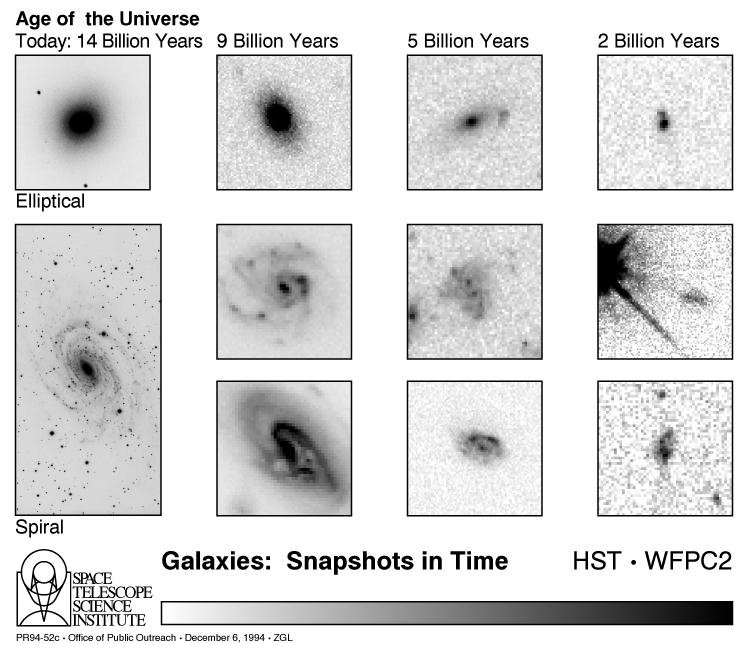
\includegraphics[width=\linewidth]{{Figures/GalaxEvC}.jpg}
	\caption[Morphological evolution of galaxies with cosmic time]{HST images of disk-like and spheroidal galaxies from $12$ billion years ago (rightmost column) to the present day (leftmost). \\ Credits:~NASA.}
	\label{fig:morpho_evol}
\end{wrapfigure}

In the local Universe, galaxies can be divided into two categories based on their shape and colour: red ellipticals and blue spirals. These are also referred to as early and late type respectively according to \shortciteA{Hubble1922},  \shortciteA{Hubble1926} classification. Even though this is true for most galaxies, we also observe a small fraction of dustier red spirals. Nevertheless, the separation is clear with very few galaxies in between the two populations. Ellipticals tend to be the most massive ($M \sim 1-5 \times 10^{11} \rm{M_\odot}$), as well as quenched, that is their Star Formation Rate (SFR) is near $0$. Most of their massive younger and bluer stars are gone (as a star's lifetime scales as its mass to the power of $-3$ or so), leaving only old red stars, which is the reason for their red colour. On the other hand, spirals are more recent, star-forming galaxies, still full of blue stars, but also smaller and lighter.
When looking at more distant parts of the Universe, say $z > 0.5$, this dichotomy is less pronounced. Giant ellipticals are more rare, those found are still forming stars and disk-like galaxies have more irregular morphologies which might be due to past merger events or unrelaxed kinematics because of a recent formation.\\

In this context, one may ask how the morphology of galaxies evolved from highly disturbed shapes $\SI{10}{Gyr}$ ago to the two distinct populations we see today. In order to answer this type of questions, we need to relate the evolution of galaxies morphology to their dynamics. Kinematical observations probe the rotation of gas embedded in  galaxies, which can give insights into the processes at play in the formation and settling of gas into discs. It is then possible to explore the impact of different physical mechanisms such as inflows, outflows, stellar feedback or merging onto these processes. This also give us access to rotation curves from which we can retrieve information about the dark matter content of galaxies, and explore the angular momentum redistribution through cosmic time. However, in order to study the co-evolution of morphological and dynamical properties with redshift, we need to rely on both morphological (radius, ellipticity) and kinematical parameters such as rotation velocity measurements or velocity dispersions. \\

Assigning a characteristic rotation velocity and a velocity dispersion to a galaxy is not a straightforward step. Generally, this is done by fitting a model onto some velocity measurement which requires spectroscopic data (3D cube or slit). Almost all galaxies are found to have flat rotation curves because of their dark matter content (except perhaps for some dwarf galaxies but these are too small to be detected at high redshift). By flat, we mean that they have a steadily rising slope from the central part until it reaches a turnover point where the curve flattens, a so-called plateau, or where it slowly decreases. In this case, the characteristic velocity which is taken into account is, most of the time, the maximum velocity at the turnover, or the plateau velocity $V_{\rm{max}}$. On the other hand, there are various ways of computing the velocity dispersion $\sigma_{\rm{v}}$, but all ultimately describe the amplitude of unordered, incoherent motion within the galaxy.\\

In the local Universe, most spirals have low velocity dispersion compared to their rotational velocity. The opposite is true for elliptical galaxies with high velocity dispersion but no significant rotation. For more distant galaxies, this might not be true any more with a much higher fraction of spiral or disk-like galaxies\footnote{We will preferentially use the terms disk-like/late-type galaxies rather than spiral as some galaxies studied in the present work do show a disk morphology without clear spiral arm patterns.} with high velocity dispersion. Usually, the parameter $V_{\rm{max}} / \sigma_{\rm{v}}$ is used to classify a galaxy as either rotationally supported ($> 1$) or as dispersion dominated ($< 1$). High redshift dispersion dominated galaxies were first discovered in the early 21st century (see \shortciteA{Glazebrook2013} for an historical perspective on the subject). These are different from the "dispersion dominated" giant ellipticals we see in the local Universe as they are less massive, more compact and yet highly star forming. Some authors hypothesized that the dispersion dominated galaxies are ancestors of the modern large ellipticals, growing by subsequent merging, or perhaps just the ancestors of the few small ellipticals we see today. Nevertheless, if there is any relation between these two populations, it is still not clear what it is. As we do not know if these dispersion dominated systems are due to unresolved rotation, investigation of the kinematics of new data with better spectral and spatial sampling is mandatory.\\

\subsubsection{An impact from the environment ?}

Theoretical modelling based on simple physics principles such as angular momentum conservation, viscous friction, dissipation of energy or gravitational instabilities can account for both the global morphology and kinematics of galaxies. And yet, state of the art N-body simulations including other components such as stellar feedback from supernovae, Active Galactic Nuclei (AGN) with their outflows, and inflows from filaments of gas in the large scale structure of the Universe have shown that these new mechanisms have more impact on the kinematics than previously thought. Moreover, seeing more disturbed morphologies and systems with high velocity dispersion at high redshift seems consistent with the hierarchical growth of dark matter haloes which drive the evolution of galaxies. In this regard, and as haloes will bound galaxies and gas together, we might expect to find a larger fraction of unrelaxed interacting and/or merging galaxies in groups and clusters than for field galaxies, that is those which do not belong to any structure. \\


Galaxies Star Formation Rate (SFR) will also depend on their redshift and their environment. This is sometimes computed through a scaling law with some gas density (generally neutral hydrogen HI) after accounting for dust attenuation, or by computing a Star Formation History (SFH) through Spectral Energy Distribution fitting techniques (requiring multi-band photometry). As stated above, the star formation is very different nowadays from the past. If we look back in time, we observe an increasing average SFR, reaching a peak around $z \sim 1.5 - 2$ and then decreasing again. This is partially linked to the fact that we observe a larger fraction of spheroidal systems with high SFR than in the local Universe. \\

Star formation only occurs when there is enough gas supplies to locally gather into collapsing clouds. Once all the gas has been consumed, the SFR is expected to quickly drop to $0$ and the galaxy becomes quenched. The question of the impact of the environment on the quenched galaxies we see today is of uttermost importance. Indeed, we expect galaxies found in groups and clusters to lie in rich hot gas environments which might be filled with inflows from filaments of gas observed in the large scale structure, or with the galaxies gas content. In the former case, this would imply higher rates of star formation in groups as there is a constant fuelling of gas. On the other hand, if the gas comes from the galaxies through physical processes such as ram pressure stripping, we should see less star forming galaxies in these regions as they might have lost a significant fraction of their content. Isolated field galaxies shall not be stripped of their gas, unless maybe if they are interacting with another galaxy at some point, though such interactions are more rare in these low density regions of the Universe. However, they will also lack inflows of gas, so we might expect to see them quench earlier than their groups and cluster counterparts. 


\subsubsection{Studying the morpho-kinematical evolution of galaxies}

\begin{wrapfigure}{l}{0.5\linewidth}
	\centering
	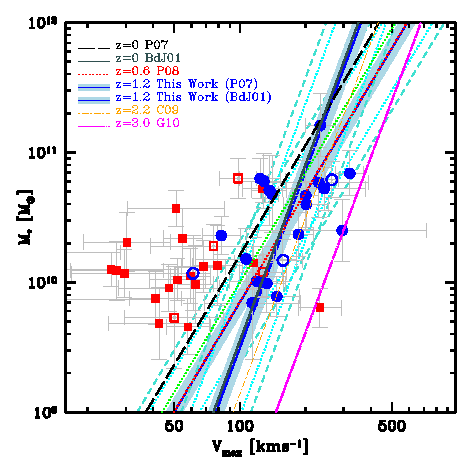
\includegraphics[width=\linewidth]{{Figures/MASSIV_TFR}.eps}
	\caption[MASSIV Tully-Fisher relation]{Stellar-mas TFR at $z \sim 1.2$ for rotating galaxies in MASSIV survey (best-fit blue line) compared against two local relations (black, $z=0$), \shortciteA{Puech2008} (red, $z \approx 0.6$), \shortciteA{Cresci2009} (orange, $z \approx 2.2$) and \shortciteA{Gnerucci2011} (magenta, $z\sim 3$).}
\end{wrapfigure}

Understanding the evolution of galaxy morphological and kinematical properties through cosmic time is not an easy task. Even though inspecting the velocity field and light profile of a spatially resolved galaxy can be useful to understand the physical mechanisms at work within, we need to perform statistics on large samples if we really want to understand the evolution of the whole galaxy population and not just of a few candidates. One of the most commonly performed morpho-kinematics comparison is the Tully-Fisher Relation (TFR) \shortcite{Tully1977}, which relates the galaxies masses to their maximum rotational velocity. This is generally compared against the aforementioned $V_{\rm{max}}/\sigma_{\rm{v}}$ ratio to distinguish between galaxies with a dominant rotation and those with dominant dispersion. 

Rotationally supported galaxies tend to lie on a sequence similar to the local TFR \shortcite{Pizagno2007}, but dispersion dominated galaxies are actually scattered around this relation \shortcite{Puech2008}. One of the current hot topics in extra-galactic astrophysics is whether or not there is any significant evolution of the stellar-mass TFR with redshift. Some authors, such as in\shortcite{Puech2008} and \shortcite{Vergani2012}, did find an evolution of the TFR zero-point, though others found no significant offset. Thus, there is not clear consensus yet on this subject. 


\newpage
\subsection{Observation techniques in astronomy}
\label{subsec:diffPhotSpec}

\subsubsection{Spectroscopy and photometry}
\label{subsubsec:photo_data}

Studying the formation and evolution of galaxies requires large datasets of objects at low and high redshifts. The two types of observation which can be carried out to answer these questions are photometry and spectroscopy. These methods originally yielded different information on the properties of galaxies such as their light distribution, their morphology or their kinematics.
Photometry provides 2D images of galaxies whose surface brightness, that is its total flux divided by its solid angle on the sky, is above the surface brightness limit imposed by the instrument limitations, but also whose size is above the instrument resolution. Depending on the band used, we can observe different galactic components, ranging from the cold, hot and ionised gas to young/old stellar populations, as well as dust.
On the other side, spectroscopy gives us information on the importance of these components with respect to the total emitted light by looking at continuum, emission and absorption lines. Galaxy spectra can contain high continuum values coming from the combination of old and young stellar populations spread through the galaxy. Detected emission lines, such as $\rm{H}{\alpha}$, $\rm{H}{\beta}$, [OII] and [OIII] doublets or $\rm{Ly}\alpha$ give us insight into the existence of gas and its ionisation, which can in turn indicate the presence of star-forming zones within the galaxy such as HII regions. Additionally, absorption lines can either show the existence of stars or potentially of intergalactic gas on the line of sight. \\
      
From 2D images we can derive morphological parameters such as the ellipticity $e = 1 - b/a$, with $b$ and $a$ the minor and major axes respectively, or some measure of a characteristic radius. Generally, it is assumed that galaxy light profiles have high degrees of symmetry. This implies that a galaxy with an inclination\footnote{We define the inclination as the angle between the plane of the galaxy and the plane of the sky, or equivalently between the normal to the plane of the galaxy and the line of sight.} $i = 0 \degree$ should have circular isophotes (lines of identical surface brightness). When elliptical isophotes are seen, which implies an elliptical shape for the galaxy, this is an indication of a non-zero inclination. Based on our definition, this translates in terms of ellipticity as

\begin{equation}
	\cos i = 1 - e
	\label{eq:inclinaison}
\end{equation}

This assumption is in fact an approximation as galaxies have more complex morphologies with central bars, spiral arms, satellite galaxies for the largest ones and potential inflows and/or outflows. It is also the case when we study galaxies which have clear disturbed morphologies due to past interactions such as merging events.  \\

In the past, measuring radii and ellipticity were generally done with a curve of growth, consisting in deriving the size and ellipticity of ellipses at different isophote levels. Nowadays, it has become common to fit galaxy light profile models onto images and to recover the morphological parameters from the best fit. One of the most commonly used is a Sérsic profile which is generally written as \shortcite{PetroRadandMag}\footnote{The original definition $I(r) \propto e^{-(r/\alpha)^{1/n}}$ from \shortciteA{Sersic1963} was modified to Eq.\,\ref{eq:SersicProfile} because of the immeasurable values $\alpha$ took in practice.} 

\begin{equation}
    \label{eq:SersicProfile}
    I(r) = I_{\rm{e}} e^{ - b_n \left ( \left  ( \frac{r}{R_{\rm{e}}}  \right )^{1/n} - 1 \right ) }
\end{equation}

where $r$ is the radial distance to the morphological centre of the galaxy, $n$ is referred as the Sérsic index, $R_e$ is the effective or half-light radius which encloses 50\% of the total luminosity, $I_e$ is the intensity at the position $R_e$ and $b_n$ is a term which ensures that $R_e$ does enclose half the total luminosity. By integrating Eq.\,\ref{eq:SersicProfile} up to infinity to recover the total luminosity $L_{\rm{tot}}$ and a second time to $R_{\rm{e}}$ so that it equals $L_{\rm{tot}}/2$, one can find the definition of $b_n$ to be such that 

\begin{equation}
2 \gamma (2n, b_n) = \Gamma (2n)
\end{equation}
with $\gamma$ and $\Gamma$ the incomplete and complete gamma functions respectively.

This equation has been widely used in different contexts because of its ability to recover two famous profiles
\begin{enumerate*}[label={(\alph*)}]
    \item an exponential disc for $n = 1$ which represents a disk-like/spiral galaxy. Here, $r$ is the radial distance in the galactic plane. Sometimes, two exponential discs are used to mimic the vertical variation of the emitted light as well as in the plane of the galaxy. 
    \item a de Vaucouleurs profile for $n = 4$ which describes early-type galaxies.
\end{enumerate*}
Depending on the author, only a single Sérsic profile with a freely varying Sérsic index can be used, as is the case for softwares such as SExtractor \shortcite{SExtractor} or GIMD2D \shortcite{GIM2D}, or a combination of a bulge and a disk, with two fixed Sérsic indices, which is the case in GALFIT \shortcite{GALFIT}. \\

Galaxies spectra can have a noisy continuum emission which can make difficult the detection of specific lines. In general, astronomers look at spectral features such as Balmer and Lyman lines, or doublets to improve the confidence in their detection. However, spectroscopes only work in a certain spectral domain, and therefore any line falling out of the instrumental range cannot be detected. When a certain component in a galaxy is observed, this requirement translates in terms of redshift through the equation $\lambda_{\rm{obs}} = \lambda_{\rm{em}} ( 1+ z)$. Thus, this implies that galaxies can only be detected in a certain redshift interval. \\

The measurement of a line is done through line fitting on a continuum subtracted spectrum. In general, an algorithm finds the redshift of a galaxy by identifying recognisable spectral features and measuring their wavelength offset from their expected rest-frame wavelength. The higher the number of detected lines, the more confidence we have in the redshift. Once this is known, each line is fitted separately with a Gaussian shaped profile from which values of the flux and the dispersion are computed. The shape and dispersion of a line is due to many factors. For galaxies spectra, deviations to Gaussian profiles are not generally considered as these are negligible and not resolved yet. The dispersion is affected both by beam smearing effects and by the velocity dispersion of the particles on the line of sight. The former corresponds to a combination of a broadening of the intrinsic velocity dispersion because of the finite instrumental spectral resolution and of the lack of spatial resolution in the central parts of the galaxies. On the other hand, the latter represents the real dispersion in the particles velocity space because of local turbulent motion induced by energy injection, for instance from supernovae. \\


\subsubsection{Long slit and early integral field spectroscopy}
\label{subsubsec:MUSE-VLT}

\begin{wrapfigure}{r}{0.5\linewidth}
	\centering
	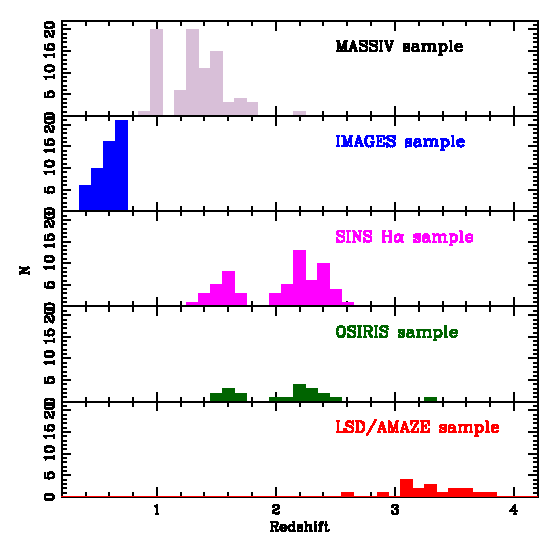
\includegraphics[width=\linewidth]{{Figures/comp_redshift_surveys}.eps}
	\caption[Redshift distribution of IFS surveys]{Comparison of the redshift distribution of the main IFS surveys mentioned in the text from \shortciteA{Contini2012}.}
\end{wrapfigure}

Before the advent of Integral Field Spectroscopy (IFS), which combines the advantages of both photometry and spectroscopy by providing a spectrum for every pixel in an image, early studies of the rotation curves of galaxies had been done with long slit spectroscopy. In this case, previously known galaxies from photometric surveys were observed with the slit of the spectrograph matching the morphological Position Angle ($\rm{PA}$) of the galaxy. This technique therefore assumed that the morphological and kinematical $\rm{PA}$ are identical, which recent studies might have proven wrong in some cases. The first resolved observation of this kind at high redshift was performed by \shortciteA{Vogt1996} with Keck Telescope. This shed the first light on the resemblance of the rotation curves between galaxies in our local Universe and those found up to $z \sim 1$. Studies of higher redshift galaxies ($2 \lesssim z \lesssim 3$) were first done on star forming UV-selected Lyman Break Galaxies (LBG), whose flux drops in the U-band because of their redshifted Lyman break.  \\

The very first 3D spectrographs observed one galaxy at a time because of the lack of a large Field of View (FoV) with good spatial resolution. In that regard, they were used for spectroscopic follow ups of already detected galaxies in photometric surveys. One of these first generation instruments was SINFONI \shortcite{Eisenhauer2003} mounted on the Very Large Telescope in Chile, working with both natural seeing and Adaptative Optics (AO). Its corresponding original survey SINS \shortcite{Schreiber2009} of $80$ objects observed from $2003$ to $2008$ was one of the first large kinematical IFS survey of its kind. During the following years, others were carried out at intermediate and high redshift. These include the OSIRIS survey \shortcite{Law2007} which observed a UV-selected sample of galaxies with OSIRIS IFS on Keck Telescope, the IMAGES survey \shortcite{Yang2008} obtained with the VLT's FLAMES-GIRAFFE multi-object integral field facility, as well as the MASSIV survey \shortcite{Contini2012} of 84 galaxies with $0.9 < z < 1.8$.


\subsubsection{New generation IFS with MUSE}

Limitations in terms of FoV, spatial sampling and surface brightness of previous IFS surveys prevented against a thorough study of galaxy kinematics in dense environments, such as clusters, as well as the inspection of low mass and low size galaxies. But with the advent of new generation spectroscopes such as the Multi Unit Spectroscopic Explorer (MUSE) \shortcite{Bacon2004} it is now possible to extend previous analyses to these two unexplored galaxy populations. MUSE is an Integral Field Unit (IFU) mounted on the VLT in Chile, observing in the visible spectrum (wavelength range from $\SI{4650}{\angstrom}$ to $\SI{9300}{\angstrom}$ with a resolution $R \sim 3000$). Its wide field-of-view of $\SI{1}{\arcmin} \times \SI{1}{\arcmin}$ and spatial sampling of $0.2 \times \SI{0.2}{arcsec^2}$ combined with its low limiting magnitude ($I_{\rm{ab}} = 25$ for $\SI{80}{h}$ of observations) allows one to perform blind surveys of galaxies in dense environments. Its high sensitivity also makes it suitable for the study of low-mass galaxies ($\log_{10} (M / \rm{M_{\odot}}) < 8.5$). Its primary purpose was to study the kinematics of medium and high redshift galaxies, and was meant to work both under seeing-limited conditions or with Adaptative Optics. The wavelength range coverage makes it particularly suitable to detect galaxies with high enough [OII] flux in the redshift domain $[0.4 , 1.4]$, but any line with high enough Signal to Noise Ratio (SNR) falling in this interval could be detected as well.